%% THE REACHABILITY MAP
%% A graphic novel screenplay
%% Format: Screenplay with panel-by-panel graphic novel annotations
%% Flyxion — Independent Author

\documentclass[11pt, letterpaper]{article}

\usepackage{palatino}
\usepackage{geometry}
\usepackage{microtype}
\usepackage{setspace}
\usepackage{titlesec}
\usepackage{enumitem}
\usepackage{xcolor}
\usepackage{mdframed}
\usepackage{tikz}
\usetikzlibrary{arrows.meta, positioning}
\usepackage{hyperref}
\usepackage{fancyhdr}
\usepackage{emptypage}

\geometry{
  top=1.0in,
  bottom=1.0in,
  left=1.5in,
  right=1.0in
}

\hypersetup{colorlinks=true, linkcolor=black, urlcolor=black}

%% ── COLOUR PALETTE ──────────────────────────────────────────────────────────
\definecolor{atlasblue}{RGB}{30, 60, 120}
\definecolor{reachred}{RGB}{160, 40, 40}
\definecolor{panelbg}{RGB}{245, 243, 238}
\definecolor{notegray}{RGB}{100, 100, 100}

%% ── TYPOGRAPHY ──────────────────────────────────────────────────────────────
\setlength{\parindent}{0pt}
\setlength{\parskip}{0.5em}

%% Scene headings: INT./EXT. in small caps, bold
\newcommand{\sceneheading}[1]{%
  \vspace{1.2em}
  {\large\bfseries\MakeUppercase{#1}}
  \vspace{0.3em}
  \hrule height 0.4pt
  \vspace{0.6em}
}

%% Action lines
\newenvironment{action}{%
  \begin{onehalfspace}\noindent
}{%
  \end{onehalfspace}
}

%% Character name above dialogue
\newcommand{\character}[1]{%
  \vspace{0.4em}
  \begin{center}
  \textbf{\MakeUppercase{#1}}
  \end{center}
}

%% Dialogue block (indented)
\newenvironment{dialogue}{%
  \begin{list}{}{%
    \setlength{\leftmargin}{1.5cm}
    \setlength{\rightmargin}{1.5cm}
  }
  \item\relax
}{%
  \end{list}
  \vspace{0.3em}
}

%% Parenthetical (stage direction within dialogue)
\newcommand{\paren}[1]{%
  \begin{list}{}{%
    \setlength{\leftmargin}{2.2cm}
    \setlength{\rightmargin}{1.5cm}
  }
  \item\relax {\itshape (#1)}
  \end{list}
}

%% Panel annotation box (graphic novel specific)
\mdfdefinestyle{panelstyle}{%
  backgroundcolor=panelbg,
  linecolor=atlasblue,
  linewidth=0.6pt,
  leftmargin=0pt,
  innerleftmargin=8pt,
  innerrightmargin=8pt,
  innertopmargin=6pt,
  innerbottommargin=6pt,
  skipabove=0.6em,
  skipbelow=0.4em,
  frametitlefont=\small\bfseries\color{atlasblue},
  frametitlerule=false,
  frametitleaboveskip=4pt,
}

\newcounter{panelcount}
\newcommand{\panel}[2][]{%
  \stepcounter{panelcount}%
  \begin{mdframed}[style=panelstyle,
    frametitle={PANEL \thepanelcount%
      \ifx&#1&\else\ —\ #1\fi}]
  \small #2
  \end{mdframed}
}

%% Caption / narrative box within panel
\newcommand{\narrbox}[1]{%
  \smallskip
  \textbf{CAPTION:} \textit{``#1''}
  \smallskip
}

%% SFX
\newcommand{\sfx}[1]{%
  \smallskip
  \textbf{SFX:} \textsc{#1}
  \smallskip
}

%% Atlas signal visual note
\newcommand{\atlassignal}[1]{%
  \smallskip
  {\color{atlasblue}\textbf{[ATLAS\,SIGNAL]:}} \textit{#1}
  \smallskip
}

%% Reachability map visual note
\newcommand{\reachmap}[1]{%
  \smallskip
  {\color{reachred}\textbf{[REACH\,MAP]:}} \textit{#1}
  \smallskip
}

%% Issue / chapter title page
\newcommand{\issuetitle}[3]{%
  \newpage
  \thispagestyle{empty}
  \vspace*{3cm}
  \begin{center}
    {\color{atlasblue}\Huge\bfseries #1}\\[0.8em]
    {\large\itshape #2}\\[2em]
    {\normalsize\color{notegray} #3}
  \end{center}
  \vspace{2cm}
  \hrule
  \newpage
  \setcounter{panelcount}{0}
}

%% Section titles (acts)
\titleformat{\section}[block]
  {\large\bfseries\color{atlasblue}\centering}
  {}
  {0em}
  {\MakeUppercase}
  [\vspace{0.2em}\hrule\vspace{0.6em}]

\titleformat{\subsection}[block]
  {\normalsize\bfseries\color{notegray}}
  {}
  {0em}
  {}

%% Page header
\pagestyle{fancy}
\fancyhf{}
\fancyhead[L]{\small\itshape Nine Parsecs}
\fancyhead[R]{\small\itshape\color{notegray}Flyxion}
\fancyfoot[C]{\small\thepage}
\renewcommand{\headrulewidth}{0.3pt}

%% ── DOCUMENT ────────────────────────────────────────────────────────────────

\begin{document}

%% ── TITLE PAGE ──────────────────────────────────────────────────────────────

\thispagestyle{empty}
\vspace*{2.5cm}

\begin{center}

{\color{atlasblue}\fontsize{36}{42}\selectfont\bfseries
NINE PARSECS}

\vspace{1.2em}

{\large\itshape A graphic novel in three volumes}

{\normalsize\color{notegray}\itshape Nine parsecs to Sector 7.\\
Standard assignment. Routine discrepancy.}

\vspace{2em}

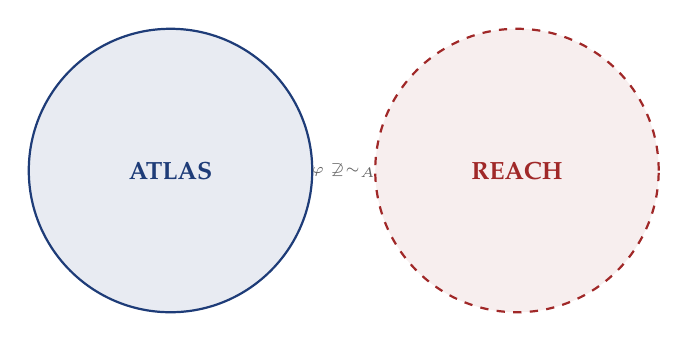
\begin{tikzpicture}
  % Two overlapping circles: Atlas map (clean) and Reachability map (messy)
  \draw[atlasblue, thick, fill=atlasblue!10]
    (-2.2,0) circle (1.8cm);
  \draw[reachred, thick, dashed, fill=reachred!8]
    (2.2,0) circle (1.8cm);
  \node[atlasblue] at (-2.2,0) {\small\bfseries ATLAS};
  \node[reachred]  at ( 2.2,0) {\small\bfseries REACH};
  \node[notegray, font=\tiny] at (0,0)
    {$\varphi \not\supseteq \sim_A$};
\end{tikzpicture}

\vspace{2em}

\begin{minipage}{0.72\textwidth}
\centering\itshape\small
``One map showed what usually happens.\\
The other showed what could still happen.''
\end{minipage}

\vspace{3em}

{\normalsize\color{notegray}
Written by \textbf{Flyxion}\\[0.3em]
Independent Author\\[0.3em]
\today}

\end{center}

\newpage

%% ── EPIGRAPH ────────────────────────────────────────────────────────────────

\thispagestyle{empty}
\vspace*{5cm}

\begin{center}
\begin{minipage}{0.6\textwidth}
\itshape
``In that Empire, the Art of Cartography attained such Perfection that the Map
of a single Province occupied the entirety of a City, and the Map of the Empire,
the entirety of a Province. In the course of Time, these Unconscionable Maps no
longer satisfied, and the Cartographers Guilds struck a Map of the Empire whose
size was that of the Empire, and which coincided point for point with it.''

\vspace{0.6em}
\raggedleft --- Jorge Luis Borges,
\textit{On Exactitude in Science}, 1946

\vspace{1.8em}

\itshape
``Every projection is a promise about which distinctions survive.\\
The question is: which promises have been kept?''

\vspace{0.6em}
\raggedleft --- Field Auditor Manual,\\
Atlas Bureau, Meridian Commonwealth,\\
\textit{Year of Synchronization 412}

\vspace{1.8em}

\itshape
``Assignment 412-7743: Sector 7, Meridian Plateau.\\
Distance from Bureau Central: nine parsecs.\\
Nature of discrepancy: administrative.\\
Estimated resolution time: three days.''

\vspace{0.6em}
\raggedleft --- Atlas Bureau Dispatch Log,\\
\textit{Year of Synchronization 412, Day 14}

\end{minipage}
\end{center}

\newpage

%% ── DRAMATIS PERSONAE ───────────────────────────────────────────────────────

\thispagestyle{empty}
\section*{Dramatis Person\ae}

\vspace{0.6em}

\textbf{BORGES} \hfill \textit{Field Auditor, Atlas Bureau. Late forties.}\\
Not a rebel. Not a hero. A professional investigator of discrepancies between
the Atlas projections and observable reality. Believes in the Atlas at the
story's opening — not fanatically, but as a craftsman believes in his tools.
His transformation is epistemological, not political.

\vspace{0.8em}

\textbf{VERA SOLIS} \hfill \textit{Senior Cartographer, Bureau of Historical Records.}\\
Fifties. Dry, precise, and unremarkable until she is not. Has spent thirty
years cataloguing the Atlas's compression history. Knows more than she says.

\vspace{0.8em}

\textbf{DIRECTOR HAAN} \hfill \textit{Head of Atlas Coherence Division.}\\
Sixties. Genuinely competent and genuinely convinced that the Atlas serves the
public good. The story's most dangerous character precisely because he is not
wrong about most things.

\vspace{0.8em}

\textbf{THE RESIDENTS OF DISTRICT 43} \hfill \textit{Collective.}\\
An entire settlement that officially does not exist as a distinct entity.
Not rebels. Farmers, mechanics, teachers, children. People living inside a
bureaucratic erasure they did not choose.

\vspace{0.8em}

\textbf{THE UNDERGROUND CARTOGRAPHERS} \hfill
\textit{``Those who mark what the Atlas no longer distinguishes.''}\\
Linguists, historians, mechanics, archivists. Their symbol is a crossed-out
projection glyph: $[\varphi]$ with a diagonal slash.

\vspace{0.8em}

\textbf{THE ATLAS} \hfill \textit{Not a character. An infrastructure.}\\
The representational system that governs the Meridian Commonwealth. Navigation,
economics, science, career assignment, risk assessment, education. No one sees
the world directly any longer. They see Atlas projections.

\newpage

%% ════════════════════════════════════════════════════════════════════════════
%% VOLUME ONE: THE DISCREPANCY
%% ════════════════════════════════════════════════════════════════════════════

\issuetitle
  {Volume One: The Discrepancy}
  {In which a field auditor investigates a mapping error\\
  and discovers it is not an error}
  {Issues 1–4\quad Pages 1–88}

%% ── ISSUE ONE ───────────────────────────────────────────────────────────────

\section*{Issue One: District 43}

\subsection*{Pages 1–4 — Arrival}

\sceneheading{Ext. Meridian Plateau — Dawn}

\panel[Wide establishing shot — double-page spread]{%
A vast plateau under a cold, pale sky. In the distance, four Atlas Towers rise
above the horizon. They are extraordinary: slender, crystalline, somewhere
between lighthouse and cathedral. Each one catches the early light differently.
They look like something mathematics might dream. Below them, a long-distance
transport crawls across empty terrain.

\narrbox{Meridian Commonwealth. Year of Synchronization 412.}
\narrbox{Nine parsecs from Bureau Central to Sector 7.}
\narrbox{Field Auditor Borges had made longer journeys. He expected this one
to take three days.}
\narrbox{The Atlas Towers were built in Year 3. No one alive remembers a world
without them.}
}

\panel[Interior of the transport — BORGES at the window]{%
BORGES sits alone in a near-empty carriage. He is not young. Heavy field coat,
worn at the elbows. A leather satchel. A battered Atlas terminal on the seat
beside him, its screen showing a regional projection map: clean lines,
colour-coded districts, confident labels.

He is looking out at the towers, not at the map.

His expression is neutral. A man doing a job he has done many times before.
On the seat beside the Atlas terminal, a dispatch slip:

\atlassignal{ASSIGNMENT 412-7743\quad SECTOR 7\quad DISTANCE: 9\,psc\quad
EST. RESOLUTION: 3 DAYS\quad NATURE: ADMINISTRATIVE DISCREPANCY}

\narrbox{Field Auditor Borges. Twenty-two years with the Bureau.}
\narrbox{He has investigated 340 discrepancies. He has resolved 340
discrepancies.}
\narrbox{Nine parsecs. Three days. Standard.}
}

\panel[Close-up on the Atlas terminal screen]{%
The map is clean and elegant. A grid of districts, each labelled. In the
centre of the region: \textbf{DISTRICT 19 (POP.\ 14,200)}. No District 43
appears anywhere on the map.

\atlassignal{DISTRICT 19 — ADMINISTRATIVE SECTOR 7 — STATUS: NOMINAL}
}

\panel[The transport slowing — a settlement visible through the window]{%
A real settlement. Dense. Lived-in. Chimneys, market stalls, a school, a
repair yard. Certainly more than fourteen thousand people.

A hand-painted sign at the entrance reads:

\textbf{DISTRICT 43 — ESTABLISHED YEAR 61}

\sfx{brakes, wind, the sound of ordinary life}
}

\newpage

\subsection*{Pages 5–8 — The Settlement}

\sceneheading{Ext./Int. District 43 — Morning}

\panel[Borges stepping off the transport, satchel in hand]{%
He looks at the sign. Looks at his terminal. Looks at the sign again.

He makes a note on a small paper pad. Old habit. The terminal records
everything, but Borges has always kept paper notes.
}

\panel[A SETTLEMENT OFFICIAL approaches — middle-aged woman, sturdy,
no-nonsense]{%
Her name badge reads: \textbf{MARET CAAL — DISTRICT 43 LIAISON}.

\character{Maret Caal}
\begin{dialogue}
Auditor. We've been expecting you.\\
We filed the discrepancy report six months ago.
\end{dialogue}

\character{Borges}
\begin{dialogue}
The Atlas logs it as District 19.
\end{dialogue}

\character{Maret Caal}
\begin{dialogue}
\paren{flatly}
Yes. We know.
\end{dialogue}
}

\panel[Walking through the settlement — wide shot showing its density]{%
It is clearly a distinct, thriving place. Its architecture is different from
the surrounding districts. Its dialect has its own cadence.

\narrbox{The Atlas had merged District 43 into District 19 eighty years ago.}
\narrbox{The merger propagated through every planning system.}
\narrbox{Roads stopped being routed here. Funding was redirected.
Teachers were not assigned.}
\narrbox{Over time, the distinction disappeared everywhere except among
the people who still lived here.}
}

\panel[Borges and Maret at a community hall — a table covered in records]{%
Old paper maps. Handwritten ledgers. Photographs. All of them showing District
43 as a distinct entity.

\character{Borges}
\begin{dialogue}
These records are genuine?
\end{dialogue}

\character{Maret Caal}
\begin{dialogue}
My grandmother was born here when it was still on the Atlas.\\
My mother was born here when it wasn't.\\
My children have never appeared in a resource allocation table.
\end{dialogue}

\paren{She sets down a ledger}

\begin{dialogue}
The Atlas says we are District 19.\\
We have always been District 43.\\
Both statements are true.\\
That is the discrepancy.
\end{dialogue}
}

\newpage

\subsection*{Pages 9–14 — The Investigation}

\sceneheading{Int. Settlement Records Room — Day}

\panel[Borges alone with the records, cross-referencing his terminal]{%
He is methodical. He has done this before. Usually the answer is clerical:
a data entry error, a boundary dispute, a legacy identifier.

He is not finding the usual answer.
}

\panel[Close on the terminal — Atlas administrative history]{%
\atlassignal{DISTRICT 19: Formed Year 332 via merger of Sectors 19-A and
19-B (formerly designated 43, 44, 45). Merger rationale: administrative
consolidation. Resource savings: 12.4\%. Planning efficiency gain: 8.1\%.}

\atlassignal{All downstream planning systems updated. Distinction preserved
in: NONE. Historical archive flag: SUPPRESSED (Year 340, Coherence Directive
7).}
}

\panel[Borges's expression — something shifting behind the professional mask]{%
He reads it again. And again.

The merger was not a mistake.

It was a decision.

A very small, very rational decision made eighty years ago by people who are
long dead.

\narrbox{12.4\% resource savings.}
\narrbox{8.1\% efficiency gain.}
\narrbox{One distinction removed.}
\narrbox{14,000 people made bureaucratically unreachable.}
}

\panel[Borges walking outside — looking up at a distant Atlas Tower]{%
It is late afternoon. The tower catches the light and scatters it in prismatic
arcs across the settlement below. Children play in those arcs of colour.

He has never thought of the towers as sinister.

He still does not.

That is what makes this difficult.
}

\panel[He opens his paper notebook and writes]{%
Close on the page, his handwriting:

\textbf{``Merger was legal. Merger was documented. Merger was rational by
every metric the Atlas uses.}

\textbf{Question: what metrics does the Atlas not use?''}

Below that, after a pause, in smaller writing:

\textbf{``District 43 is reachable. It is only unreachable inside the
projection.''}
}

\panel[Evening — Borges at a window, the settlement lit up below]{%
Ordinary life. A bakery closing. A repair shop open late. Someone teaching
children to read under a lamp.

All of it outside the Atlas.

All of it happening anyway.

\narrbox{340 discrepancies resolved.}
\narrbox{This one was different.}
\narrbox{The others had been errors.}
\narrbox{This was a feature.}
}

\newpage

\subsection*{Pages 15–22 — The Transmission}

\sceneheading{Int. Borges's Field Office — Night}

\panel[Borges filing his initial report — terminal screen]{%
He types carefully. He is a professional. He documents everything.

\atlassignal{FIELD REPORT 412-7743\\
Auditor: Borges\\
Location: Sector 7, Meridian Plateau\\
Status: DISCREPANCY CONFIRMED}

\atlassignal{Finding: The settlement designated District 43 in pre-332
records exists as a physically and socially distinct entity. Current Atlas
designation as District 19 subsector is a consequence of Year 332
administrative merger, not an error.}

\atlassignal{Recommendation: CLASSIFICATION REVIEW. Possible systemic
pattern — see attached notes.}
}

\panel[A reply arrives almost immediately — unusual]{%
\atlassignal{FROM: Director Haan, Atlas Coherence Division\\
TO: Auditor Borges\\
PRIORITY: STANDARD}

\atlassignal{Report received. Merger Year 332 was conducted under
Coherence Directive 4, legally binding. No review required. Close file.
Return to Bureau.}
}

\panel[Borges reads it twice]{%
He closes the reply.

Opens his paper notebook.

Writes one word:

\textbf{``Why?''}
}

\panel[He does not close the file]{%
He opens his terminal again and begins pulling historical records.

Not about District 43.

About every merger since Year 100.

There are 847 of them.

\narrbox{A field auditor investigating a discrepancy has broad access
to historical records.}
\narrbox{He had never needed it before.}
\narrbox{He needed it now.}
}

\panel[Montage — pages of records scrolling, night deepening]{%
Each merger shows the same pattern:

\textbf{Resource savings.}\\
\textbf{Efficiency gains.}\\
\textbf{Distinction removed.}\\
\textbf{Historical archive: SUPPRESSED.}

\narrbox{847 mergers.}
\narrbox{847 distinctions removed.}
\narrbox{847 rational decisions.}
}

\panel[Final panel of Issue One — Borges at the window, dawn arriving]{%
The Atlas Tower on the horizon catches the first light. Beautiful. Perfect.
Mathematical.

He looks at it for a long time.

\narrbox{The Atlas was not wrong.}
\narrbox{It predicted everything it was designed to predict.}
\narrbox{The question Borges was beginning to ask was different.}
\narrbox{Not: what does it predict?}
\narrbox{But: what does it erase?}
}

\newpage

%% ── ISSUE TWO ───────────────────────────────────────────────────────────────

\section*{Issue Two: The History of Collapse}

\subsection*{Pages 23–30 — Bureau of Historical Records}

\sceneheading{Int. Atlas Bureau, Central Archive — Day}

\panel[Wide shot — the Archive]{%
Enormous. Cathedral ceilings. Rows of physical records alongside terminals.
The Bureau of Historical Records occupies three subterranean floors of the
Central Atlas Tower.

VERA SOLIS is at her desk in the centre of it all: small, precise, surrounded
by three open ledgers and a terminal she appears to be ignoring.

\narrbox{Vera Solis. Chief Archivist. Thirty years with the Bureau.}
\narrbox{She had requested a transfer nine times. It had been denied nine times.}
\narrbox{She had stopped requesting.}
}

\panel[Borges arriving at her desk — she does not look up]{%
\character{Borges}
\begin{dialogue}
I sent a request for access to pre-332 compression records.
\end{dialogue}

\character{Vera Solis}
\begin{dialogue}
\paren{still not looking up}
I know. I approved it.\\
No one else would have.
\end{dialogue}
}

\panel[She finally looks up — direct, assessing]{%
\character{Vera Solis}
\begin{dialogue}
District 43?
\end{dialogue}

\character{Borges}
\begin{dialogue}
You know it?
\end{dialogue}

\character{Vera Solis}
\begin{dialogue}
I know 847 of them.\\
\paren{a pause}
Sit down, Auditor.
\end{dialogue}
}

\panel[She spreads a large old paper map across the desk]{%
It is different from any Atlas map Borges has seen. Denser. More detailed.
Filled with small notations in faded ink.

\character{Vera Solis}
\begin{dialogue}
This is a Year 100 administrative map.\\
Before the Great Consolidation.
\end{dialogue}

\character{Borges}
\begin{dialogue}
I don't recognise most of these designations.
\end{dialogue}

\character{Vera Solis}
\begin{dialogue}
No. You wouldn't.\\
They no longer exist in the Atlas.\\
They still exist in the world.
\end{dialogue}
}

\newpage

\subsection*{Pages 31–40 — The Pattern}

\sceneheading{Int. Archive — Continuous}

\panel[Vera unrolling a second, older map — even denser]{%
\character{Vera Solis}
\begin{dialogue}
Every generation, the Atlas becomes more efficient.\\
Fewer categories. Broader classes. Smoother predictions.
\end{dialogue}

\character{Borges}
\begin{dialogue}
That is its purpose.
\end{dialogue}

\character{Vera Solis}
\begin{dialogue}
Yes. That is exactly its purpose.
\end{dialogue}

\paren{She sets down the map and looks at him}

\begin{dialogue}
Borges. What does the Atlas not predict?
\end{dialogue}
}

\panel[Borges, considering]{%
\character{Borges}
\begin{dialogue}
Noise. Outliers. Statistical anomalies.\\
Events in the tail of the distribution.
\end{dialogue}

\character{Vera Solis}
\begin{dialogue}
Events in the tail.\\
\paren{quietly}
Yes.
\end{dialogue}
}

\panel[She pulls out a ledger and opens it to a specific page]{%
\character{Vera Solis}
\begin{dialogue}
In Year 180, there was a drought in what was then District 43.\\
The Atlas had no category for it — the region had been merged into
a coastal administrative zone. All drought preparedness resources
went to the coast.
\end{dialogue}

\character{Borges}
\begin{dialogue}
I don't see that in any official records.
\end{dialogue}

\character{Vera Solis}
\begin{dialogue}
No. You wouldn't.\\
The affected population was, by that point, administratively inside
the coastal zone. The drought occurred in a place that did not
officially exist as a drought-prone region.\\
\paren{pause}
Seven hundred people.
\end{dialogue}
}

\panel[Long silence — Borges processes this]{%
\character{Borges}
\begin{dialogue}
The merger was rational.
\end{dialogue}

\character{Vera Solis}
\begin{dialogue}
Every individual merger was rational.\\
The Atlas was optimising.\\
It simply did not know it was optimising away certain futures.
\end{dialogue}
}

\panel[She closes the ledger]{%
\character{Vera Solis}
\begin{dialogue}
The Atlas is an extraordinary prediction machine.\\
It is very good at telling you what usually happens.
\end{dialogue}

\paren{She looks out a high window toward a Tower}

\begin{dialogue}
What it cannot tell you\\
is what is still possible.\\
Those are not the same thing.
\end{dialogue}
}

\newpage

\subsection*{Pages 41–50 — The Reachability Layer}

\sceneheading{Int. Deep Archive — Restricted Access — Later}

\panel[Vera leads Borges into a lower level of the Archive]{%
Older. Darker. Physical storage — actual printed records in acid-free boxes.
The terminals down here are a different generation.

\narrbox{Sub-level 3. Access requires Archivist clearance.}
\narrbox{Borges had never been below Sub-level 1.}
}

\panel[Vera retrieving a specific box — methodical, she has done this before]{%
\character{Vera Solis}
\begin{dialogue}
The original Atlas architecture had two layers.
\end{dialogue}

\character{Borges}
\begin{dialogue}
I know. The predictive layer and the administrative layer.
\end{dialogue}

\character{Vera Solis}
\begin{dialogue}
Three layers.
\end{dialogue}

\paren{She sets the box on a reading table}

\begin{dialogue}
There was a third.
\end{dialogue}
}

\panel[She opens the box — original engineering documents, Year 3–20]{%
Detailed. Mathematical. Dense.

\character{Vera Solis}
\begin{dialogue}
The founders called it the Reachability Layer.\\
Its purpose was different from prediction.\\
While the predictive layer modelled what would probably happen,\\
the reachability layer modelled what could still happen.
\end{dialogue}

\character{Borges}
\begin{dialogue}
What is the difference?
\end{dialogue}
}

\panel[Vera drawing a quick diagram on paper — two overlapping circles]{%
One circle: clean, solid border. Label: \textbf{PREDICTION}.

One circle: larger, dashed border. Label: \textbf{REACHABILITY}.

The prediction circle is inside the reachability circle.

\character{Vera Solis}
\begin{dialogue}
The predictive layer tracks what is likely.\\
The reachability layer tracks what is accessible.\\
Every likely thing is accessible.\\
Not every accessible thing is likely.
\end{dialogue}
}

\panel[Borges staring at the diagram]{%
\character{Borges}
\begin{dialogue}
The rare things.
\end{dialogue}

\character{Vera Solis}
\begin{dialogue}
The rare things. The tail events. The low-probability futures.\\
The reachability layer preserved them.\\
Not because they were probable.\\
Because they were \textit{possible.}\\
And some of them mattered enormously.
\end{dialogue}
}

\panel[Final panel of the sequence — close on one of the founding documents]{%
A formal technical notation in Year-3 script. Borges leans closer to read it.

Translated into modern script as a caption:

\narrbox{``The predictive layer learns from the past. The reachability layer
models the future's shape. Both are required. Neither is sufficient alone.
A civilization that loses its reachability layer does not collapse
immediately. It simply becomes, over time, less able to reach its own
possibilities.'' --- Chief Engineer Maren, Year 12}

\character{Borges}
\begin{dialogue}
\paren{quietly}
When was it removed?
\end{dialogue}

\character{Vera Solis}
\begin{dialogue}
Year 89. Resource constraints.\\
The reachability layer consumed three times the compute of the
predictive layer.\\
The Efficiency Council voted 11 to 2 to shut it down.\\
\paren{a pause}
The decision was documented as an ``architectural optimisation.''
\end{dialogue}
}

\newpage

%% ── ISSUE THREE ─────────────────────────────────────────────────────────────

\section*{Issue Three: The Underground Cartographers}

\subsection*{Pages 51–60 — The Symbol}

\sceneheading{Ext./Int. Various Locations — Day and Night}

\panel[Borges walking through the city — he notices something]{%
On a wall. Small. Easily missed.

A symbol: the Atlas projection glyph, $\varphi$, crossed by a diagonal slash.

He has seen it before. He thought it was graffiti.

Now he stops.
}

\panel[The same symbol — in three other places Borges passes]{%
On a doorframe. Chalked on a pavement stone. Carved into the base of a public
bench.

\narrbox{He had walked past it hundreds of times.}
\narrbox{He had never looked at it.}
}

\panel[Borges photographing the symbol with his terminal]{%
\atlassignal{IMAGE SEARCH: No matching symbols in Atlas cultural registry.}
\atlassignal{Recommendation: Flag as unregistered cultural expression.
Classification: NOISE.}

\paren{He looks at the screen for a long moment, then closes it.
He takes out his paper notebook and sketches the symbol by hand.}
}

\panel[Vera's office — Borges showing her the sketch]{%
She glances at it.

Does not react.

\character{Borges}
\begin{dialogue}
You've seen this before.
\end{dialogue}

\character{Vera Solis}
\begin{dialogue}
\paren{after a pause}
Yes.
\end{dialogue}
}

\panel[A long look between them]{%
\character{Borges}
\begin{dialogue}
The Atlas doesn't know about them.
\end{dialogue}

\character{Vera Solis}
\begin{dialogue}
The Atlas classified them as noise thirty years ago.\\
Once something is classified as noise,\\
it stops being tracked.\\
\paren{quietly}
That is how they prefer it.
\end{dialogue}
}

\newpage

\subsection*{Pages 61–70 — The Meeting}

\sceneheading{Int. Repair Workshop — Night}

\panel[Borges being led through back streets by Maret Caal]{%
\character{Borges}
\begin{dialogue}
You know them.
\end{dialogue}

\character{Maret Caal}
\begin{dialogue}
District 43 has been outside the Atlas for eighty years.\\
You find resources where you can.
\end{dialogue}
}

\panel[A workshop — machine tools, maps covering every wall]{%
The maps are extraordinary. Hand-drawn, printed, scratched on metal, woven
into fabric. All of them dense. All of them filled with distinctions the Atlas
no longer makes.

Six people waiting. Different ages, backgrounds, professions. A mechanic.
A linguist. A retired teacher. An archivist (not Vera). A young engineer.
A very old woman whose hands are permanently ink-stained.

\narrbox{The Underground Cartographers.}
\narrbox{They do not call themselves that.}
\narrbox{They call themselves: People Who Mark What the Atlas No Longer
Distinguishes.}
\narrbox{The name is too long for most conversations.}
}

\panel[The ink-stained woman speaks — she is ELDER NAESS]{%
\character{Elder Naess}
\begin{dialogue}
A Bureau auditor.\\
\paren{she studies him}
You found the pattern.
\end{dialogue}

\character{Borges}
\begin{dialogue}
I found a discrepancy.
\end{dialogue}

\character{Elder Naess}
\begin{dialogue}
Yes. That is where it always begins.
\end{dialogue}
}

\panel[She moves to a large wall map]{%
It is a composite — hundreds of sources, decades of work. Every merged
district, every suppressed distinction, every administrative collapse marked
in red.

\reachmap{The wall map covers 847 mergers and approximately 3,200 secondary
collapses. The red marks form a pattern: systematic, concentric, accelerating
over time.}

\character{Elder Naess}
\begin{dialogue}
The Atlas predicts what is likely.\\
We map what is still reachable.\\
\paren{she traces the red marks slowly}
These are the things that are no longer reachable.\\
Not because they became impossible.\\
Because they became invisible.
\end{dialogue}
}

\panel[Borges, absorbing this]{%
\character{Borges}
\begin{dialogue}
The Atlas is not wrong.\\
Its predictions are accurate.
\end{dialogue}

\character{Elder Naess}
\begin{dialogue}
Completely accurate. Yes.\\
For everything it still distinguishes.\\
\paren{turning to face him}
That is the problem, Auditor.\\
A map that only shows roads it recognises\\
will correctly predict every journey that uses those roads.\\
It will tell you nothing\\
about the territories it has stopped mapping.
\end{dialogue}
}

\newpage

\subsection*{Pages 71–80 — The Proposition}

\sceneheading{Int. Workshop — Later}

\panel[The young engineer — TESSIAN — spreading technical documents]{%
He is in his late twenties. Nervous energy. Brilliant in a way that has not
yet learned to hide itself.

\character{Tessian}
\begin{dialogue}
We have been rebuilding it.\\
The Reachability Layer.\\
From the original Year-3 documents.
\end{dialogue}

\character{Borges}
\begin{dialogue}
You have the original documents?
\end{dialogue}

\character{Tessian}
\begin{dialogue}
Vera Solis copied them.\\
Over thirty years.\\
One page at a time.
\end{dialogue}
}

\panel[Borges sitting with this information]{%
\character{Borges}
\begin{dialogue}
What does it show?\\
The reachability layer.\\
What does it actually show?
\end{dialogue}

\character{Tessian}
\begin{dialogue}
\paren{pulling up a prototype display}
Everything the Atlas still predicts, but also —\\
the branches.\\
The low-probability futures.\\
The things that are possible but unlikely.\\
The distinctions that matter for crisis response,\\
for adaptation, for reaching places\\
the current trajectory would never take you.
\end{dialogue}
}

\panel[The display activates — two maps side by side]{%
On the left: an Atlas projection. Clean, confident, well-labelled.

On the right: the reachability prototype. The same region. But denser.
Filled with faint lines, alternative pathways, branching structures.
It looks like a river delta viewed from above, or the fine structure of a leaf.

\reachmap{The reachability map has approximately eight times the information
density of the Atlas projection. Much of it is faint — low-probability — but
present. The missing distinctions are visible as a kind of texture.}

\character{Borges}
\begin{dialogue}
\paren{quietly}
It's not a better prediction.\\
It's a different object entirely.
\end{dialogue}

\character{Tessian}
\begin{dialogue}
Yes. Exactly that.
\end{dialogue}
}

\panel[Elder Naess watching Borges]{%
\character{Elder Naess}
\begin{dialogue}
The Atlas tells you where you are going.\\
The reachability layer tells you where you could still go.\\
\paren{a pause}
A civilization that has only one of those\\
does not know the difference.\\
Eventually it begins to believe\\
that only what is likely\\
is what is possible.
\end{dialogue}
}

\panel[Borges and Elder Naess — the exchange]{%
\character{Borges}
\begin{dialogue}
I traveled nine parsecs to investigate a discrepancy.
\end{dialogue}

\character{Elder Naess}
\begin{dialogue}
\paren{quietly}
Nine parsecs to reach us.\\\\
How far is the Atlas from the territory it claims to map?
\end{dialogue}

\paren{No one answers. The two maps glow on the display beside them.}
}

\panel[Borges looking at the two maps for a long time]{%
No speech bubble.

Just a man who has spent twenty-two years resolving discrepancies
understanding, perhaps for the first time, what discrepancy actually means.

\narrbox{340 discrepancies resolved.}
\narrbox{This one could not be resolved.}
\narrbox{It could only be understood.}
}

\newpage

%% ── ISSUE FOUR ──────────────────────────────────────────────────────────────

\section*{Issue Four: Director Haan}

\subsection*{Pages 81–88 — The Hearing}

\sceneheading{Int. Atlas Bureau, Director's Suite — Day}

\panel[Wide shot — the Director's office, high in the Central Tower]{%
Floor to ceiling windows. The city spread out below. Three Atlas Towers
visible on the horizon.

DIRECTOR HAAN behind a clean desk. A tall man. Methodical. Calm. He has the
manner of someone who has thought carefully about everything and arrived at
correct conclusions.

\narrbox{Director Haan had joined the Atlas Bureau at twenty-two.}
\narrbox{He believed in it the way an architect believes in load-bearing
structures.}
\narrbox{He was not wrong about most things.}
\narrbox{That was the difficulty.}
}

\panel[Borges across the desk — formal, controlled]{%
\character{Director Haan}
\begin{dialogue}
You did not close the District 43 file.
\end{dialogue}

\character{Borges}
\begin{dialogue}
No.
\end{dialogue}

\character{Director Haan}
\begin{dialogue}
I instructed you to close it.
\end{dialogue}

\character{Borges}
\begin{dialogue}
I found additional relevant material.
\end{dialogue}
}

\panel[Haan opens a file — a copy of Borges's extended report]{%
\character{Director Haan}
\begin{dialogue}
You are claiming that the merger programme constitutes a systematic
pattern of what you call ``admissibility failure.''\\
\paren{he reads from the report}
``The Atlas projection does not merely fail to represent certain
reachable states. By acting on the projection, the Bureau actively
narrows the reachable futures of the affected populations.''\\
\paren{he sets the file down}
That is a very serious claim.
\end{dialogue}
}

\panel[Haan, leaning back — not hostile, genuinely engaging]{%
\character{Director Haan}
\begin{dialogue}
Borges. The Atlas has governed this Commonwealth for four hundred years.\\
In that time: no famines. No wars of the type that destroyed the
pre-Atlas civilizations. Life expectancy doubled. Resources reach
ninety-three percent of the population within viable timeframes.\\
You are telling me this system is failing.
\end{dialogue}

\character{Borges}
\begin{dialogue}
I am telling you it is optimising.\\
Those are different claims.
\end{dialogue}
}

\panel[Haan, a flicker of something — not anger, closer to genuine interest]{%
\character{Director Haan}
\begin{dialogue}
Explain that.
\end{dialogue}

\character{Borges}
\begin{dialogue}
The Atlas is very good at producing the futures it expects.\\
Seven hundred people died in a drought in Year 180\\
because the region they lived in had been merged out of the
drought-preparation category.\\
The Atlas did not predict the drought incorrectly.\\
It had simply stopped tracking whether that region could experience one.
\end{dialogue}
}

\panel[Long silence — Haan at the window, looking at the city]{%
\character{Director Haan}
\begin{dialogue}
\paren{quietly, more to himself than to Borges}
We cannot track everything.\\
The reachability layer was removed because it was computationally
intractable.\\
The founders made a choice.\\
\paren{turning back}
Every generation makes the same choice.\\
Efficiency over completeness.\\
It has served us well.
\end{dialogue}

\character{Borges}
\begin{dialogue}
It has served the people inside the projection well.\\
\paren{a pause}
District 43 is not inside the projection.
\end{dialogue}
}

\panel[Final panel of Volume One — Haan and Borges, facing each other]{%
Haan does not order Borges to close the file.

He does not threaten him.

He says:

\character{Director Haan}
\begin{dialogue}
I will read your full report, Borges.\\
\paren{very quietly}
I am not certain you are wrong.\\
I am not certain it matters.
\end{dialogue}

\narrbox{Volume One ends here.}
\narrbox{Not with a conspiracy revealed.}
\narrbox{Not with a system condemned.}
\narrbox{With two people who understand the problem differently}
\narrbox{and are not sure which understanding is actionable.}
}

\newpage

%% ════════════════════════════════════════════════════════════════════════════
%% VOLUME TWO: THE COMPRESSION
%% ════════════════════════════════════════════════════════════════════════════

\issuetitle
  {Volume Two: The Compression}
  {In which the history of collapse is mapped\\
  and what was lost begins to be named}
  {Issues 5–8\quad Pages 89–176}

\subsection*{Synopsis — Volume Two}

\begin{action}
Volume Two moves between the past and present. Borges, now working with the
Underground Cartographers under unofficial tolerance from Haan, begins the
process of auditing not a single discrepancy but the entire history of
compression. Each issue introduces a different mode of collapse: geographic
(merging of places), linguistic (merging of dialects and categories), scientific
(merging of risk classifications), and social (merging of professions and
identities).

Each collapse was rational. Each was documented. Each removed a distinction.
Each made certain futures less accessible.

The central visual motif of Volume Two is the two maps side by side: the
Atlas map becoming progressively cleaner and more compressed over the decades,
while the reachability map, reconstructed from the Underground Cartographers'
archive, shows the corresponding loss of branching structure — futures that
were possible and are no longer being modelled.

The emotional centre of Volume Two is the discovery of the Year 89 vote. Borges
obtains the original transcript of the Efficiency Council meeting at which the
reachability layer was shut down. It is eleven to two. The two dissenting votes
left written records. Borges reads them and does not know what to do with what
he learns: the people who voted to shut down the reachability layer were not
wrong about the resource constraints. The people who voted against were not
wrong about what would be lost.

Both sides were right about the things they were right about.

That is the most Strugatsky-like moment in the manuscript.
\end{action}

\newpage

%% ════════════════════════════════════════════════════════════════════════════
%% VOLUME THREE: THE SECOND MAP
%% ════════════════════════════════════════════════════════════════════════════

\issuetitle
  {Volume Three: The Second Map}
  {In which nothing is overthrown\\
  and something is restored}
  {Issues 9–12\quad Pages 177–264}

\subsection*{Synopsis — Volume Three}

\begin{action}
Volume Three does not resolve the conflict between the Atlas and the
reachability layer. It does not replace one with the other. The outcome is
smaller and more durable than that.

Borges succeeds in one thing: he proves, formally and publicly, that the Atlas
is not reality. Not wrong. Not evil. But not the same as the territory it maps.

The final issue opens on a classroom. A standard Atlas-curriculum lesson on
geographic organisation. The teacher is following the standard Atlas projection.
Then she pauses and calls up a second display.

The two maps appear side by side for the first time in a Commonwealth
classroom in three hundred years.

The students look at them.

A student asks: ``Which one is the real map?''

The teacher answers:

``One tells you what usually happens. The other tells you what is still
possible.''

She does not say the Atlas is wrong. She does not say the reachability map
is right. She says they are different objects that answer different questions.

The final panel zooms out to show Borges standing at the back of the room.
No speech bubble. No caption. Just a man who resolved 340 discrepancies and
one pattern, watching two maps share a wall for the first time.

A faint smile.

The end.
\end{action}

\newpage

%% ── VISUAL DESIGN NOTES ─────────────────────────────────────────────────────

\section*{Visual Design Notes for the Artist}

\subsection*{The Atlas Towers}

The Atlas Towers should be beautiful. This is not negotiable. Dystopian
stories frequently make the sources of their problem ugly or sinister; this one
must not. The Towers are elegant, mathematical structures somewhere between a
lighthouse, an observatory, and a cathedral. They are places where people get
married, where children learn to read, where scientists do their best work.
The problem the story describes is not created by anything sinister. It was
created by rational decisions. This must be visible in the architecture.

Suggested design language: crystalline geometry, arcing light, mathematical
precision. The Towers should look like something built by people who loved
knowledge and were very good at their jobs.

\subsection*{The Two Maps}

The Atlas Map and the Reachability Map are the story's central visual objects.
They should be clearly distinct at a glance but clearly related.

\textbf{Atlas Map}: Clean. Confident. Saturated colour. Clear district
boundaries. Well-labelled. Beautiful in the way good graphic design is
beautiful. A document that inspires trust.

\textbf{Reachability Map}: Denser. Softer. Branching structures — like a river
delta, a leaf's vascular system, or a probability tree. Many pathways shown
in fainter ink, indicating low probability but real possibility. It looks
like the Atlas map plus a layer of potential beneath it. When the two are
shown side by side, the Reachability Map should feel like the Atlas map with
its shadows restored.

\subsection*{The Underground Cartographers' Symbol}

The symbol $[\varphi]$ with a diagonal slash should be small and handmade
wherever it appears. Not monumental. Not threatening. The size of something
scratched by one person who wanted to mark that this place was more than the
projection said it was.

\subsection*{Colour Grammar}

\begin{itemize}[leftmargin=1.5em, itemsep=0.2em]
  \item {\color{atlasblue}\textbf{Atlas Blue}} — institutional confidence,
    predictive accuracy, the official world
  \item {\color{reachred}\textbf{Reachability Red}} — the branching futures,
    the preserved distinctions, what remains possible
  \item \textbf{Archival Ochre} — old records, the pre-compression world,
    Vera's documents
  \item \textbf{Warm Grey} — ordinary life in both the Atlas-visible and
    Atlas-invisible settlements
\end{itemize}

\subsection*{Tone}

The story should feel like a procedural mystery that gradually reveals itself
to be a philosophical meditation. The visual pacing of Volume One is slow and
documentary. Volume Two is denser and more archival. Volume Three opens out
into something closer to ordinary life — schools, markets, children — as the
stakes become clarified.

The ending panel should feel earned, quiet, and only slightly hopeful. Not a
victory. A beginning.

\newpage

%% ── APPENDIX: THEMATIC NOTES ────────────────────────────────────────────────

\section*{Appendix: Thematic Notes}

\subsection*{On Maps and Territories}

The central premise is the inverse of Borges's \textit{On Exactitude in
Science}. Where that story imagined a map so detailed it became the territory,
this story imagines a map so compressed that it can no longer represent the
territory's possibilities. Both failures are failures of the relationship
between representation and reality. The first is a failure of economy. The
second is a failure of fidelity to what remains reachable.

\subsection*{On the Atlas as a Character}

The Atlas is not a villain. It is not malfunctioning. It is doing exactly
what it was designed to do, with great competence. The problem is not that
the Atlas is bad at predicting. The problem is that prediction and reachability
are different things, and a civilization that has only a prediction layer has
no formal way to know what it has stopped being able to reach.

This is important for the reader's experience: the story should never feel
like an argument against prediction, planning, or systematic knowledge. It
is an argument that prediction alone is insufficient --- that reachability
is a prior condition, not a competitor.

\subsection*{On the Strugatsky Influence}

The Strugatsky brothers, particularly in \textit{Prisoners of Power} and
\textit{Roadside Picnic}, wrote about societies shaped by forces they could not
fully understand and individuals who had to act within those societies without
the comfort of moral clarity. The present story follows that model. Borges is
not a hero. Haan is not a villain. The Efficiency Council of Year 89 was not
wrong. The two dissenting votes were not wrong either. Everyone is operating
within the limits of what they can know and what they can choose given those
limits.

The Strugatskyan element is not the dystopia. It is the absence of a clean
resolution. The reachability layer cannot simply be restored. Three hundred
years of compression cannot simply be reversed. What can happen is smaller
and more important: a civilization can learn, again, to hold two maps.

\subsection*{On the Formal Correspondence}

For readers of the associated theoretical work, the graphic novel \textit{Nine Parsecs} can be read
as a dramatisation of the admissibility distortion framework. The Atlas
represents a learned projection $\varphi$ optimised for predictive accuracy.
The mergers represent admissibility-violating collapses --- pairs of states
(districts, populations, categories) identified despite possessing different
reachability sets. The Reachability Layer is a visualisation of the admissibility
quotient $\mathcal{X}/{\sim_A}$ that the Atlas projection has departed from.
Director Haan represents the genuinely correct observation that the predictive
layer works well for everything it still models --- that
$D_A^{\pi}(\varphi) \approx 0$ under the current policy. Borges's report
argues for the structural distortion: $D_A^{\mathrm{struct}}(\varphi) \gg 0$
in the regions the current policy no longer visits. The classroom ending is
not a proof. It is the first time two maps --- the predictive quotient and the
admissibility quotient --- share the same wall.

\bigskip

\noindent\textbf{End of Treatment.}

\end{document}
